\section{Metodologia} % Seções são adicionadas para organizar sua apresentação em blocos discretos, todas as seções e subseções são automaticamente exibidas no índice como uma visão geral da apresentação, mas NÃO são exibidas como slides separados.

\begin{frame}
	\frametitle{Metodologia}
	\small
	
	\vfill
	\begin{columns}
		\begin{column}{0.60\textwidth}
			\begin{itemize}
				\item Confecção de um \textit{dataset} curado por especialistas sobre um GEM que tenha ampla cobertura no repositório BIGG e artigos científicos.
				\item Experimento comparativos de \textbf{três fases}, alterando-se \textbf{apenas o mecanismo de recuperação} entre elas , o que isola o efeito das \textbf{camadas simbólicas} sobre as métricas de qualidade do RAG.
				\item Ferramentas e LLMs \textit{open-source} serão utilizados.
				\item O \textit {framework open-source} RAGAS será utilizado para gerar as métricas de avaliação
			\end{itemize} 
		\end{column}
		\begin{column}{0.40\textwidth}
			\begin{figure}[H]
				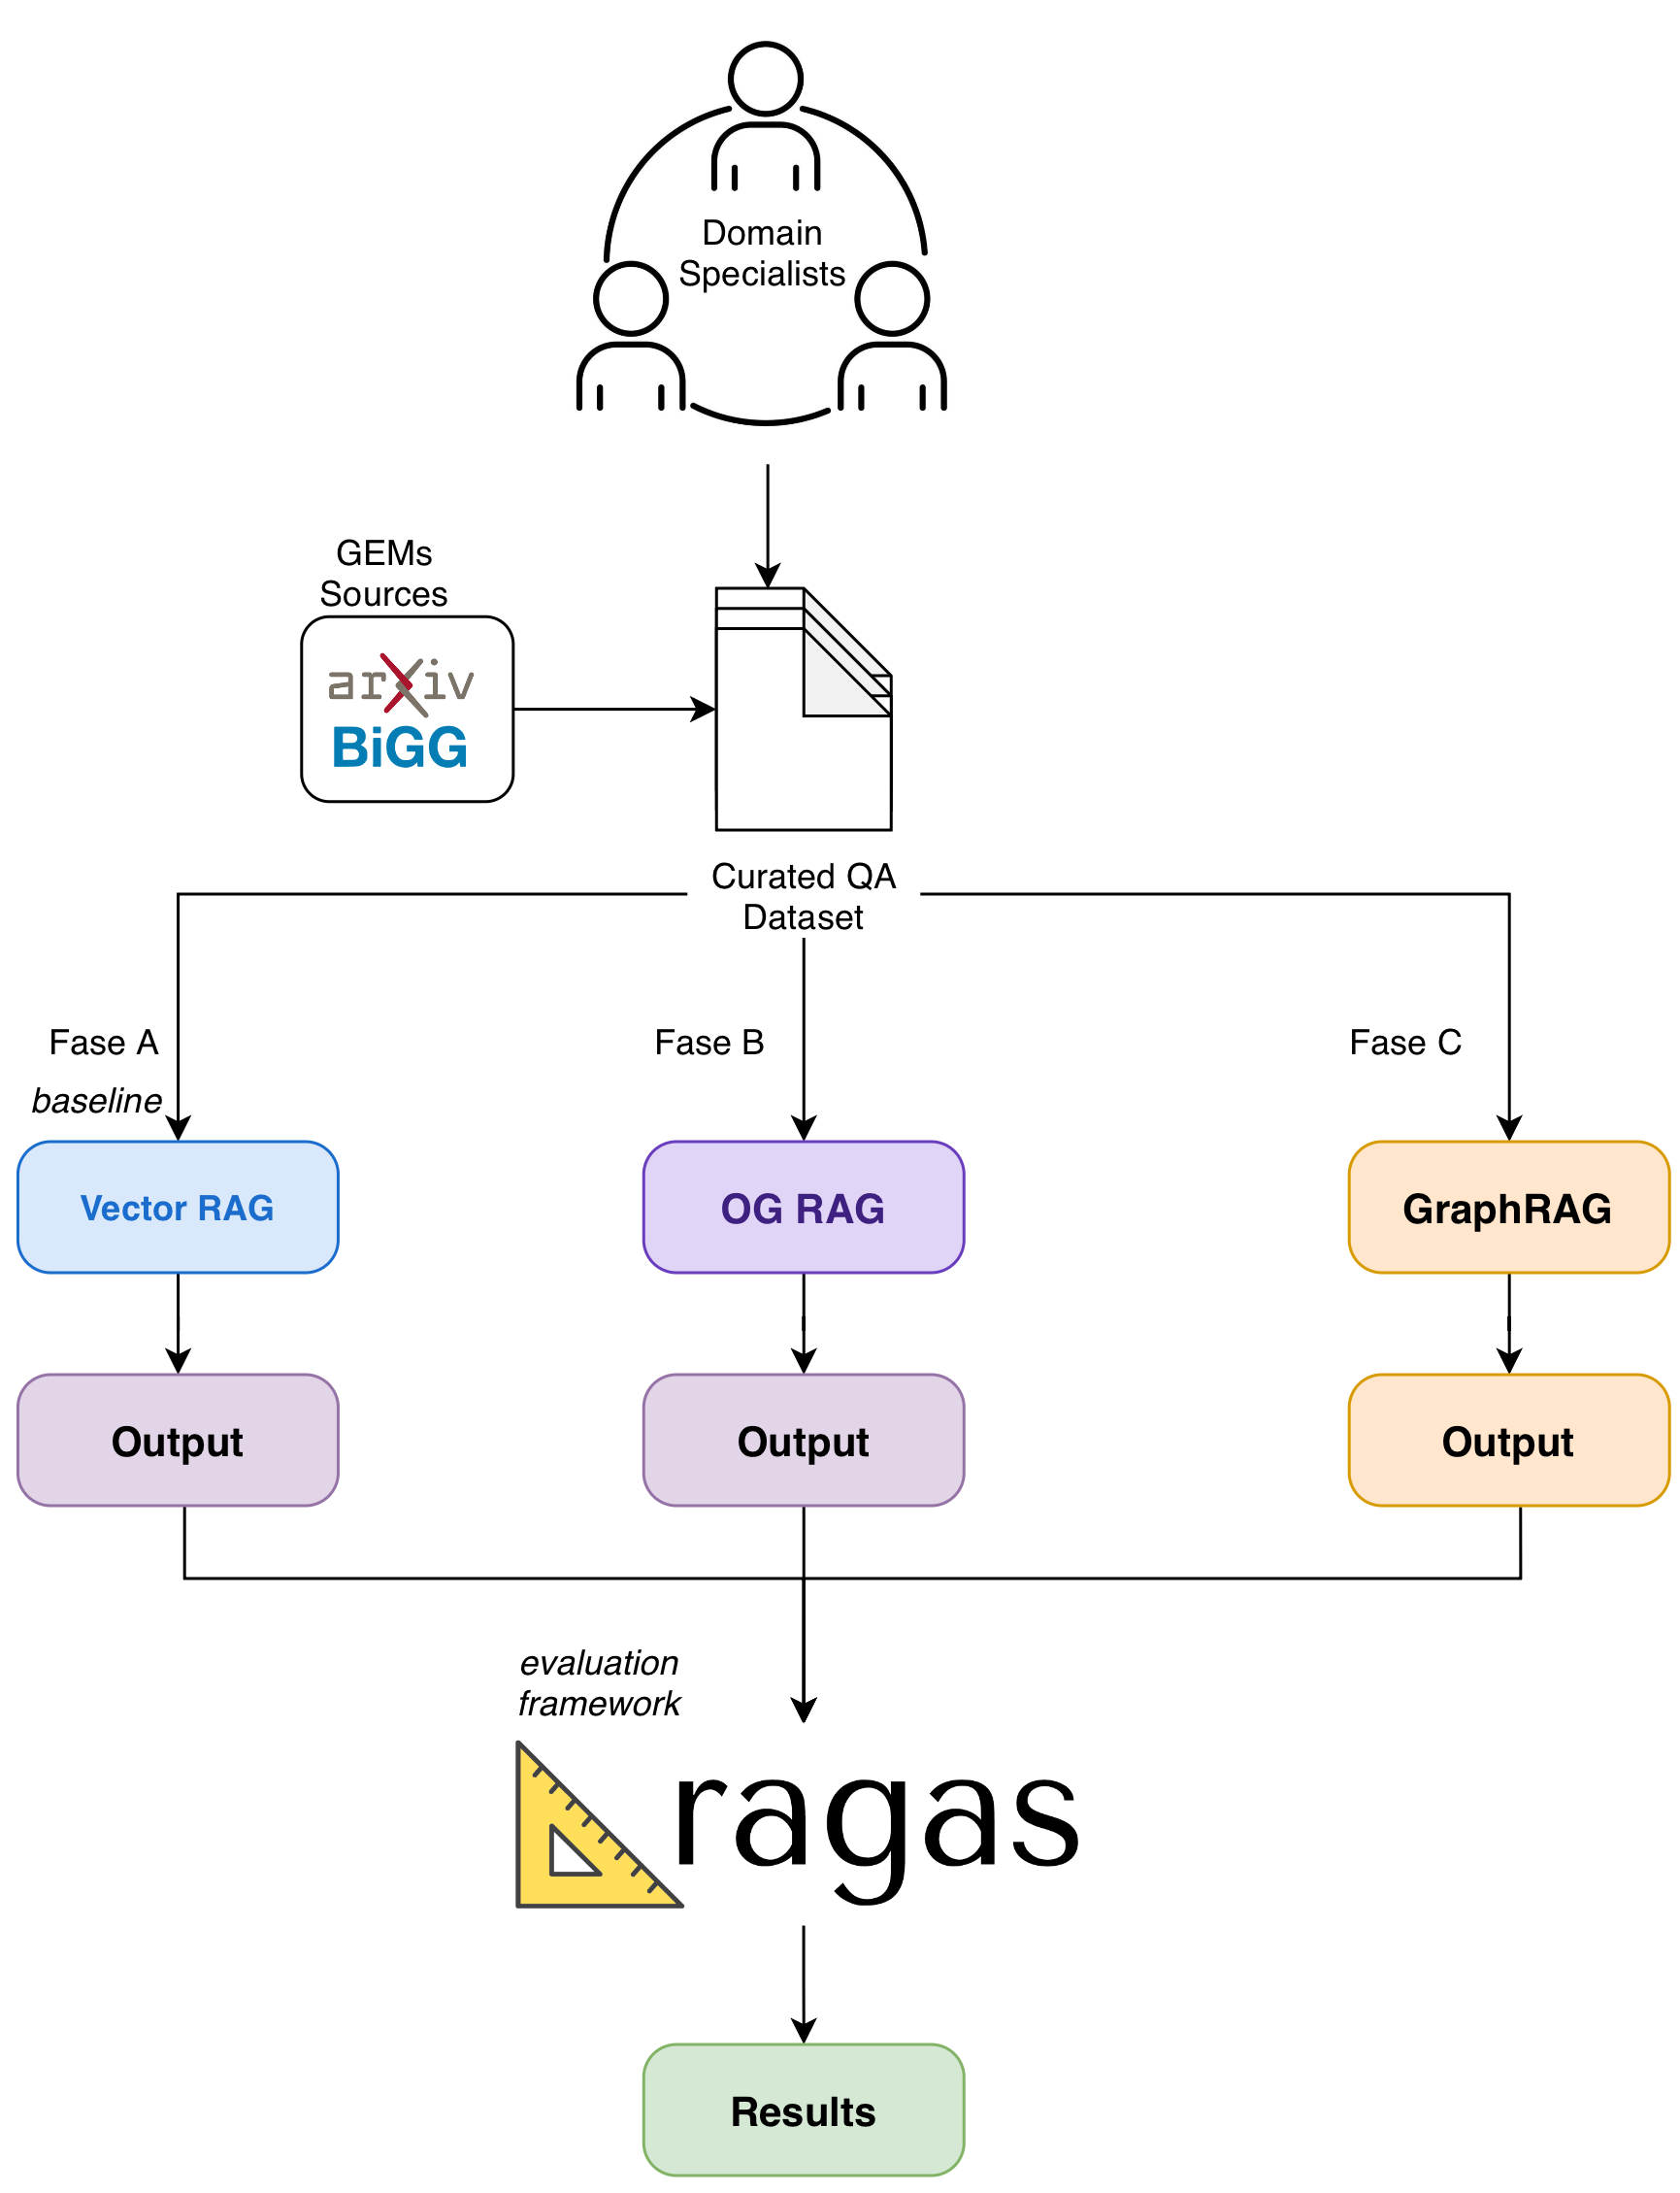
\includegraphics[width=\linewidth]{img/metodologia.png}
			\end{figure}
		\end{column}
	\end{columns}
\end{frame}